\documentclass[12pt]{article}

\usepackage{xeCJK}
\usepackage{ctex}
\usepackage{pdfpages}
\usepackage{titlesec}
\usepackage{fontspec}
\usepackage{booktabs}
\usepackage{graphicx}
\usepackage{float}
\usepackage{subfigure}
\usepackage{listings}
\usepackage{amsmath}
\usepackage{amssymb}
\usepackage{geometry}
\usepackage{xcolor}
\usepackage{fancyhdr}
\usepackage[hidelinks]{hyperref}
\usepackage{algpseudocode}
\usepackage{algorithm}
\usepackage{bm}
\usepackage{threeparttable}
\usepackage{textcomp}

\graphicspath{ {assets/} }

\pagestyle{fancy}
\fancyhf{}
\renewcommand{\headrulewidth}{0pt}
\fancyfoot[L]{程序设计实践报告}
\fancyfoot[R]{\thepage}
\fancyfoot[C]{}

\geometry{a4paper,footskip=4cm}

\titleformat{\title}
{\centering\bfseries \zihao{4} \heiti}
{\thesection}
{1em}
{}

\titleformat{\section}
{\centering \color{xblue} \bfseries \zihao{4} \heiti}
{\thesection}
{1em}
{}

\titleformat{\subsection}
{\raggedright\bfseries \zihao{-4} \heiti}
{\thesubsection}
{1em}
{}

\titleformat{\subsubsection}
{\raggedright\bfseries \zihao{-4} \heiti}
{\thesubsubsection}
{1em}
{}

\definecolor{xblue}{RGB}{0,0,148}

\setmonofont{CascadiaCode.ttf}

\lstset{
    backgroundcolor=\color{white},
    keywordstyle=\color{blue},
    numberstyle=\color[RGB]{0,192,192},
    commentstyle=\color[RGB]{0,96,96},
    stringstyle=\color[RGB]{128,0,0},
    columns=fullflexible,
    breaklines=true,
    captionpos=b,
    tabsize=4,
    numbers=left,
    frame=single,
    basicstyle=\ttfamily
}

\urlstyle{same}

\floatname{algorithm}{算法}
\renewcommand{\algorithmicrequire}{\textbf{输入:}}
\renewcommand{\algorithmicensure}{\textbf{输出:}}

\makeatletter
\newenvironment{breakablealgorithm}
  {% \begin{breakablealgorithm}
    \begin{center}
      \refstepcounter{algorithm}% New algorithm
      \hrule height.8pt depth0pt \kern2pt% \@fs@pre for \@fs@ruled
      \parskip 0pt
      \renewcommand{\caption}[2][\relax]{% Make a new \caption
        {\raggedright\textbf{\fname@algorithm~\thealgorithm} ##2\par}%
        \ifx\relax##1\relax % #1 is \relax
          \addcontentsline{loa}{algorithm}{\protect\numberline{\thealgorithm}##2}%
        \else % #1 is not \relax
          \addcontentsline{loa}{algorithm}{\protect\numberline{\thealgorithm}##1}%
        \fi
        \kern2pt\hrule\kern2pt
     }
  }
  {% \end{breakablealgorithm}
     \kern2pt\hrule\relax% \@fs@post for \@fs@ruled
   \end{center}
  }
\makeatother

\begin{document}

\begin{titlepage}

\newgeometry{top=2cm,left=2cm}

\parbox[c]{8cm}{
    
\includegraphics[width=8cm]{hdu.png}
}

\setlength{\parindent}{0pt}
\centering
\vfill
{\zihao{-0} \heiti \textcolor{xblue}{程序设计实践报告}\par}
\vspace{10pt}
{\zihao{-2} \heiti 递归和试探回溯\par}
\vfill
{\large \heiti 卓越学院\par
计算机科学英才班\par
鲍溶\par
23060827\par
}
\vfill
\restoregeometry

\end{titlepage}

\renewcommand\contentsname{\textcolor{xblue}{目录}}
    \tableofcontents
\clearpage
\setcounter{page}{1}

\section{问题描述}

从下列分治法和回溯法应用中各选一题, 完成解题, 提交解题报告.

分治法:
\begin{itemize}
    \item 快速排序非递归算法实现;
    \item 汉诺塔问题非递归算法实现;
    \item 连通块问题非递归算法实现.
\end{itemize}

回溯法:
\begin{itemize}
    \item 迷宫问题;
    \item 马踏棋盘;
    \item 离散背包问题;
    \item 人员组合问题.
\end{itemize}

在本报告中, 我们选择快速排序非递归算法实现与迷宫问题求解.

\section{主要算法}

\subsection{迭代快速排序}

算法 \ref{algo_quicksort_iter} 描述了迭代快速排序算法. 该算法通过维护一个显式的栈实现状态保存与恢复. 我们记 $\mathsf{Push}(\cdot, \cdot)$ 与 $\mathsf{Pop}(\cdot)$ 为压入与弹出操作, $\mathsf{Empty}(\cdot)$ 为判断栈是否为空的操作.

\begin{breakablealgorithm}
\caption{末主元迭代快速排序.}
\label{algo_quicksort_iter}
\begin{algorithmic}[1]
\Require 待排序数组 $\bm{a},$ 全序关系 $\preceq,$ 待排序数组长度 $n.$
\Ensure 排序完成的数组.
\State 初始化栈 $s$
\State $l \gets 1$
\State $h \gets n$
\State $\mathsf{Push}(s, (l, h))$
\While{$\lnot \mathsf{Empty}(s)$}
    \State $(l, h) \gets \mathsf{Pop}(s)$
    \State $p \gets \bm{a}[h]$
    \State $i \gets l$
    \For{$j \gets l \dots h$}
        \If{$\bm{a}[j] \preceq p$}
            \State $\mathsf{Swap}(\bm{a}[i], \bm{a}[j])$
            \State $i \gets i + 1$
        \EndIf
    \EndFor
    \State $\mathsf{Swap}(\bm{a}[i], \bm{a}[h])$
    \State $p \gets i$
    \If{$p - 1 \ge l$}
        \State $\mathsf{Push}(s, (l, p - 1))$
    \EndIf
    \If{$p + 1 < h$}
        \State $\mathsf{Push}(s, (p + 1, h))$
    \EndIf
\EndWhile
\State 销毁栈 $s$
\State \Return $\bm{a}$
\end{algorithmic}
\end{breakablealgorithm}

\subsection{回溯法迷宫探索}

算法 \ref{algo_maze_explore} 描述了利用回溯法实现的迷宫探索. 同样, 我们记 $\mathsf{Push}(\cdot, \cdot)$ 与 $\mathsf{Pop}(\cdot)$ 为压入与弹出操作, $\mathsf{Empty}(\cdot)$ 为判断栈是否为空的操作, $\mathsf{Top}(\cdot)$ 为获取栈顶元素的操作.

\begin{breakablealgorithm}
\caption{回溯法迷宫探索.}
\label{algo_maze_explore}
\begin{algorithmic}[1]
\Require 迷宫 $M.$
\Ensure 是否能够找到一条可行路线.
\State 初始化栈 $s$
\State $P \gets \mathrm{NULL}$
\State $\mathsf{Push}(s, \text{初始坐标})$
\While{$\lnot \mathsf{Empty}(s)$}
    \State $P \gets \mathsf{Top}(s)$
    \State 标记 $P$ 为已探索过的道路
    \For{$P' \gets \{ P\ \text{的右、 左、 上、 下方坐标}\}$}
        \If{$P'$ 在迷宫内部, 且为未探索过的道路}
            \State $\mathsf{Push}(s, P')$
            \State 跳过剩余检测, 继续 \textbf{while} 循环的下一迭代
        \EndIf
    \EndFor
    \State $\mathsf{Pop}(s)$
\EndWhile
\If{$P$ 为终点}
    \State \Return 能够找到一条可行路线
\Else
    \State \Return 无法找到一条可行路线
\EndIf
\end{algorithmic}
\end{breakablealgorithm}

\section{实验设计}

\subsection{迭代快速排序}

由于在专题任务 1 中, 我们对快速排序算法的实现已经采用了迭代法, 故不再重复具体过程. 相关实现代码见附录和专题任务 1.

\subsection{回溯法迷宫探索}

我们使用 C 语言为回溯法迷宫探索算法实现了一个简单的终端 ASCII-art 图形交互界面. 该程序有基于 \texttt{ncurses} \cite{bib_ncurses} 的 Unix\textsuperscript{\textregistered} 分支和基于 \texttt{PDCurses} \cite{bib_pdcurses} 的 Windows\textsuperscript{\textregistered} 分支. 实现了跨平台的终端图形界面. 该程序的源代码见附录 \ref{appendix_source_code}. 给定迷宫大小后, 用户可以使用键盘对迷宫结构进行编辑, 并在编辑完成后以每步为单位观察探索过程.

\section{结果分析}

\subsection{迭代快速排序}

迭代法快速排序的分析见专题任务 1.

\subsection{回溯法迷宫探索}

如图 \ref{fig_screenshot_mazerwin} 所示, 我们使用 \texttt{mazer\_win} 程序对一个 $20 \times 20$ 的迷宫进行了探索. 该样例说明本程序能够实现稳定且用户友好的图形交互.

\begin{figure}[H]
    \centering
    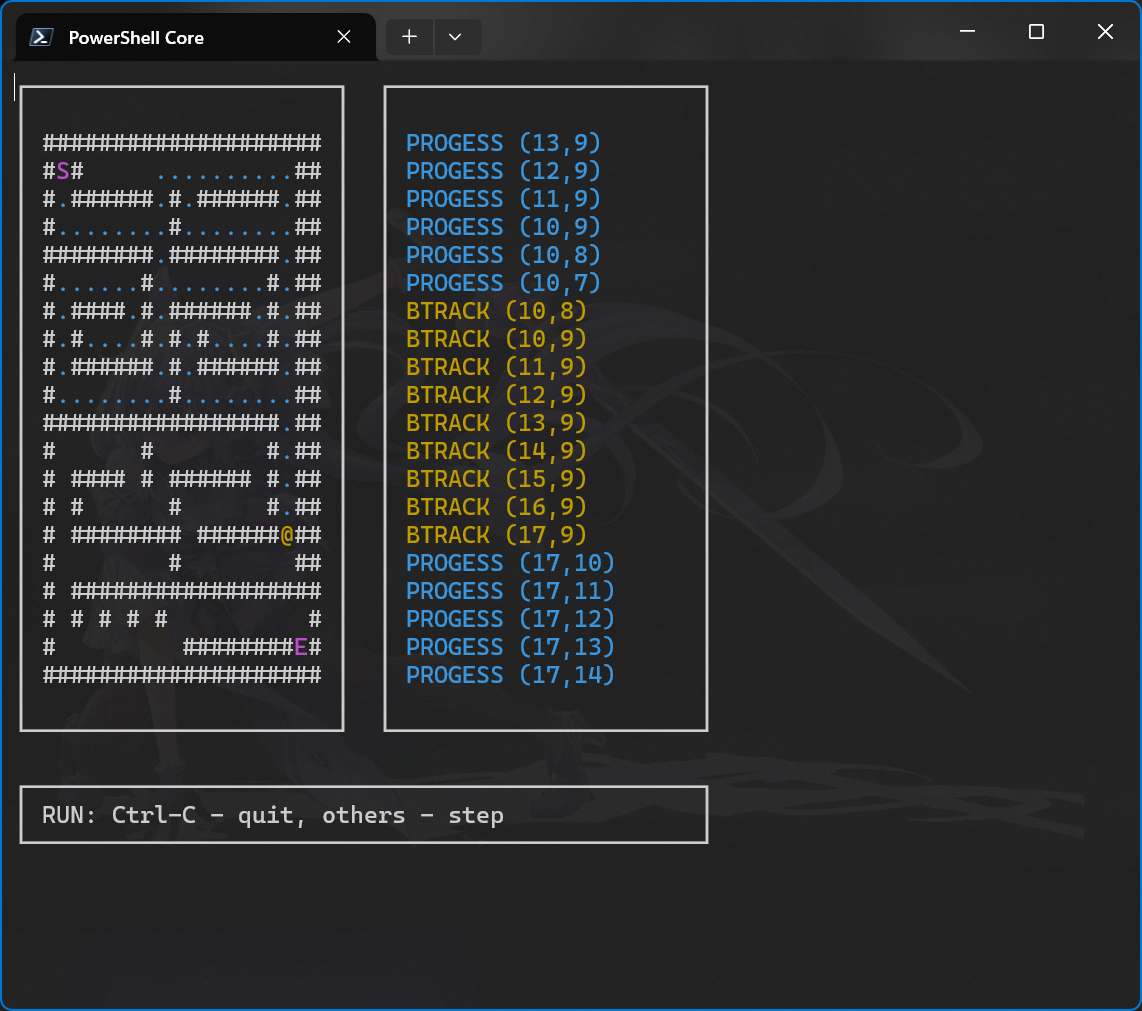
\includegraphics[scale=0.4]{screenshot_mazerwin_v010}
    \caption{\texttt{mazer\_win} 某一次运行的终端截图}
    \label{fig_screenshot_mazerwin}
\end{figure}

\section{小结}

本文实现了迭代快速排序和回溯法迷宫探索两种算法, 并以可交互的形式对后者结果进行展示.  实验中, 作者对递归与试探回溯的原理有了更深刻的理解, 对如何稳定地通过控制台进行图形交互也有了更深入的认识.

\begin{thebibliography}{}

\bibitem{bib_ncurses} NCURSES - New Curses \textbf{[OL]}. https://invisible-island.net/ncurses/
\bibitem{bib_pdcurses} PDCurses - a curses library for environments that don't fit the termcap/terminfo model. \textbf{[OL]}. https://pdcurses.org/

\end{thebibliography}

\appendix

\section{附录: 算法实现}

\subsection{迭代快速排序}

\begin{lstlisting}[language=C]
static algo_errno_t partition_highpivot(void *arr, size_t size, size_t low, size_t high, comp_t comp, uint64_t threshold, uint64_t *counter, size_t *out_result) {
    uint8_t *arr_ = arr;

    uint8_t *pivot = arr_ + high * size;
    size_t i = low - 1;

    for (size_t j = low; j <= high; j++) {
        COUNTER_INC_AND_CHECK(*counter, threshold);
        if (comp(arr_ + j * size, pivot) < 0) {
            i++;
            swap_bytes(arr_ + i * size, arr_ + j * size, size);
        }
    }
    swap_bytes(arr_ + (i + 1) * size, arr_ + high * size, size);
    *out_result = i + 1;

    return OK;
}

static algo_errno_t quicksort_highpivot_impl(void *arr, size_t size, size_t low, size_t high, comp_t comp, uint64_t threshold, uint64_t *counter) {
    size_t *stack = (size_t *)malloc(sizeof(size_t) * (high - low + 1));
    if (stack == NULL) {
        return INTERNAL_ERR;
    }
    
    int64_t top = -1;

    stack[++top] = low;
    stack[++top] = high;

    while (top >= 0) {
        high = stack[top--];
        low = stack[top--];

        size_t p;
        ALGO_ERRNO_UNWRAP_FREE(partition_highpivot(arr, size, low, high, comp, threshold, counter, &p), stack);

        if (!((p - 1 - low) & (1ull << (sizeof(size_t) * 8 - 1)))) {
            stack[++top] = low;
            stack[++top] = p - 1;
        }

        if ((p + 1 - high) & (1ull << (sizeof(size_t) * 8 - 1))) {
            stack[++top] = p + 1;
            stack[++top] = high;
        }
    }

    free(stack);

    return OK;
}

algo_errno_t quicksort_highpivot(void *arr, size_t count, size_t size, comp_t comp, uint64_t threshold, uint64_t *out_counter) {
    if (count <= 1) {
        return OK;
    }

    return quicksort_highpivot_impl(arr, size, 0, count - 1, comp, threshold, out_counter);
}
\end{lstlisting}

\subsection{回溯法迷宫探索}

\lstinputlisting[language=C]{../src/model.c}

\section{附录: 源代码可见性}
\label{appendix_source_code}

本报告中, 迷宫探索程序的 C 语言源代码可于 \url{https://github.com/CSharperMantle/mazer} 和 \url{https://github.com/CSharperMantle/mazer_win} 处获得. 迭代快速排序的 C 语言源代码可于 \url{https://github.com/CSharperMantle/sort_algo_perf} 处获得. 上述代码均可在 BSD 3-Clause 许可证的条件与条款下使用. 关于授权协议的具体信息, 详见上述 URL.

\end{document}
